\begin{frame}{Intersection of 7-branes in F-theory}
\begin{figure}[h]
\centering
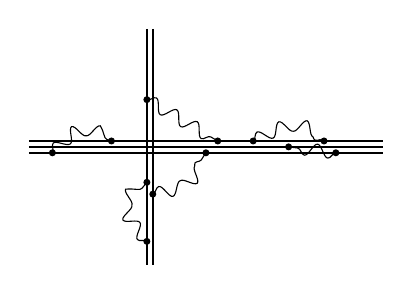
\begin{tikzpicture}[scale=.15]
% horizontal lines
\draw[ thick] (0,9.5) -- (30,9.5);
\draw[ thick] (0,10) -- (30,10);
\draw[ thick] (0,10.5) -- (30,10.5);
% vertical lines
\draw[ thick] (10,20) -- (10,0);
\draw[ thick] (10.5,20) -- (10.5,0);
% strings
\filldraw (10.5,6) circle [radius=7pt];
\filldraw (15,9.5) circle [radius=7pt];
\draw[decorate,decoration={snake,amplitude=.8mm,segment length=3mm}] (10.5,6) .. controls (13,6.5) .. (15,9.5);
\filldraw (10,14) circle [radius=7pt];
\filldraw (16,10.5) circle [radius=7pt];
\draw[decorate,decoration={snake,amplitude=.8mm,segment length=3mm}] (10,14) -- (16,10.5);

\filldraw (10,2) circle [radius=7pt];
\filldraw (10,7) circle [radius=7pt];
\draw[decorate,decoration={snake,amplitude=.8mm,segment length=3mm}] (10,2) .. controls (8,4.5) .. (10,7);

\filldraw (2,9.5) circle [radius=7pt];
\filldraw (7,10.5) circle [radius=7pt];
\draw[decorate,decoration={snake,amplitude=.8mm,segment length=3mm}] (2,9.5) .. controls (4,11.5) .. (7,10.5);

%\filldraw (5,9.5) circle [radius=7pt];
%\filldraw (9,9.5) circle [radius=7pt];
%\draw[decorate,decoration={snake,amplitude=.8mm,segment length=3mm}] (5,9.5) .. controls (7,8) .. (9,9.5);

\filldraw (19,10.5) circle [radius=7pt];
\filldraw (25,10.5) circle [radius=7pt];
\draw[decorate,decoration={snake,amplitude=.8mm,segment length=3mm}] (19,10.5) .. controls (22,12) .. (25,10.5);

\filldraw (26,9.5) circle [radius=7pt];
\filldraw (22,10) circle [radius=7pt];
\draw[decorate,decoration={snake,amplitude=.8mm,segment length=3mm}] (26,9.5) -- (22,10);
\end{tikzpicture}
\end{figure}
\begin{itemize}
\item[$\rightarrow$] In the intersection locus charged (anti-)chiral multiplets are localized.
\end{itemize}
\end{frame}

\begin{frame}{Overview geometric objects}
\begin{table}
\centering
\begin{tabular}{p{0.35\textwidth}|p{0.35\textwidth}|c}
Geometry&Physics&Dimension\\
\toprule
open strings on branes & gauge bosons & $\dim_{\C} = 2$\\\midrule
intersection of two branes & matter & $\dim_{\C} = 1$\\\midrule
intersection of two matter curves & interaction & $\dim_{\C} = 0$\\
\bottomrule
\end{tabular} 
\end{table}
\end{frame}